\documentclass[11pt, letterpaper]{article}
\usepackage[margin=0.5in]{geometry}
\usepackage{graphicx}

\begin{document}

\title{Suffix String Alignment}
\author{Tavin Turner}
\maketitle

\section{Introduction}
Seeing DNA sequence alignment as a string processing problem, we can see matching a pattern to some index in a sequence as equivalent to matching that pattern to the prefix of all of the string's suffixes. In so doing, we unravel a variety of suffix data structures to achieve sequence alignment – namely, suffix tries, trees, and arrays. Suffix tries and trees both index every suffix from the starting root connecting nodes by extending sequences – in tries, this sequence is one character, while trees use the substring until another divergence in the suffixes. Suffix arrays, on the other hand, sort the indices that a suffix begins at in alphabetical order of those suffixes, enabling a binary search procedure. Theoretical statistics for these data structures can be found in Table \ref{tab:thoretical}.

\begin{table}[h]
    \centering
    \begin{tabular}{|c|c|c|c|c|c|}
        \hline
        Model & Gen. Runtime & Gen. Memory & Size & Align. Runtime & Align. Memory \\ \hline
        Suffix trie & $O(n^2)$ & $O(n^2)$ & $O(n^2)$ & $O(m)$ & $O(1)$ \\
        Suffix tree & $O(n^2)$ & $O(n^2)$ & $O(n^2)$ & $O(m)$ & $O(1)$ \\
        Suffix array & $O(n\log n)$ & $O(n^2)$ & $O(n)$ & $O(\log n)$ & $O(1)$ \\\hline
    \end{tabular}
    \caption{Theoretical statistics of suffix string alignment data structures.}
    \label{tab:thoretical}
\end{table}

\section{Results}
In line with the theoretical expectations, suffix trie took significantly more time than suffix array to generate, although the performance difference of single-character edges is apparent even in construction, where the otherwise identical suffix tree has such dramatically lower construction run time that it is invisible when charted against the suffix trie~(Figure \ref{fig:generation}). Unexpectedly, both suffix trie and suffix tree appear significantly memory-efficient in practical construction than the suffix array, likely since the suffix array explicitly stores every suffix during sorting before discarding later.

With increasing query size, the suffix tree and suffix array appear roughly equivalent in performance over the experimental query range, although the suffix tree empirically shows the theoretical runtime increase with query size~(Figure \ref{fig:alignment}). The suffix trie, however, takes up to ten times as long as the other approaches, with less consistent trends of performance over query size. Interestingly, although all of the algorithms show their $O(1)$ theoretical alignment space~(Table \ref{tab:thoretical}), the suffix array take significantly more memory overall~(Figure \ref{fig:alignment}), since it has to index the string separately for each character, which is not stored with the array.

%%%%% Add your experiment here %%%%

\begin{figure}[h] \centering
    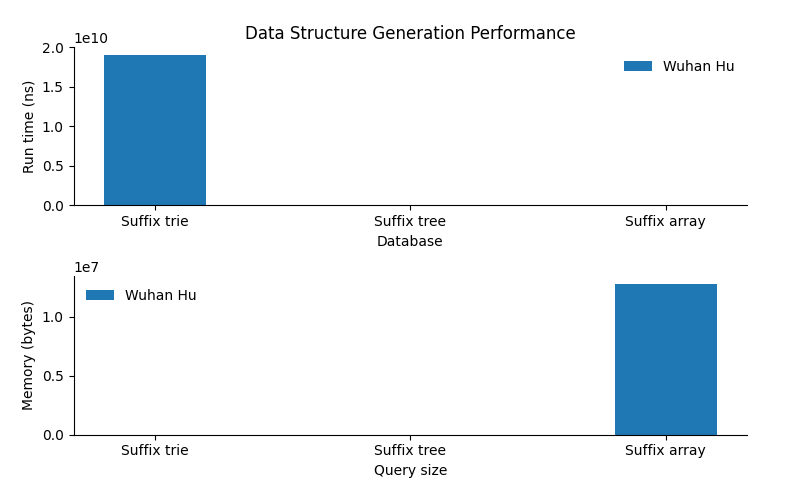
\includegraphics[width=0.6\textwidth]{wuhana_q5-30-5_n5_generation.png}
    \caption{The empirical runtime and memory usage of generating suffix tries, trees, and arrays for the first 5000 characters of the Wuhan Hu dataset.}
    \label{fig:generation}
\end{figure}

\begin{figure}[h] \centering
    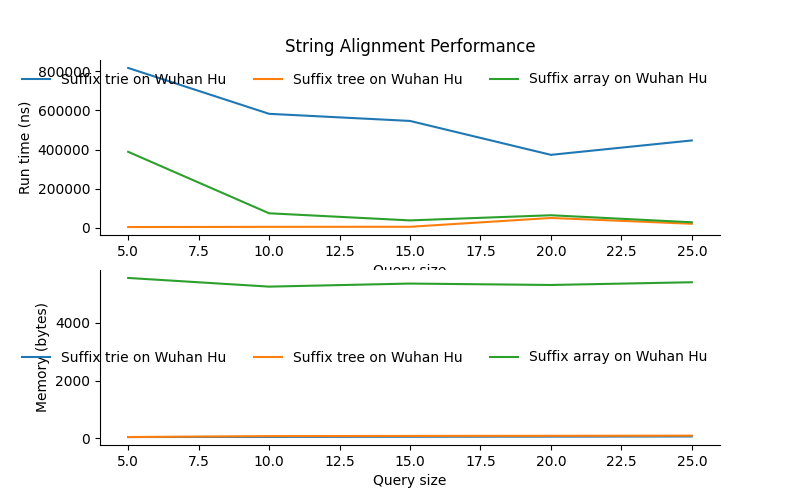
\includegraphics[width=0.6\textwidth]{wuhana_q5-30-5_n5_alignment.png}
    \caption{The empirical runtime and memory usage of aligning strings of various lengths to the first 5000 characters of the Wuhan Hu dataset with suffix tries, trees, and arrays.}
    \label{fig:alignment}
\end{figure}

%%%% Add your figure here %%%%

\section{Methods}

\subsection{Suffix trie}
The suffix trie is constructed from a text $T$ by taking each suffix $S=T[i:]$ in increasing length and searching the existing trie for each character iteratively until a branch does not exist fo the suffix, which it then creates new successive branches for each remaining character afterward. Searching the suffix trie is a simple traversal of the trie by character.

\subsection{Suffix tree}
Like the suffix trie, the suffix tree is constructed from a text $T$ by taking each suffix $S$ in increasing length and searching the tree, but instead searches through the suffix left-to-right with each edge, which may be a substring, until a misalignment is found or a leaf is reached, at which point the tree truncates the preceding branch at the misalignment and gives it two children: the remainder of the existing branch and the new remaining substring. Searching the suffix tree takes the same method as its construction.

\subsection{Suffix array}
The suffix array is constructed by sorting the indices of each suffix by the suffix in alphabetical order. To search the array, a binary search for the lowest index before a lower-order suffix than the pattern is found, then a binary search for the highest index before a higher-order suffix than the pattern is found.

\subsection{Empirical comparison}

We evaluated the performance of the suffix string search algorithms considering five pattern sizes of 5, 10, 15, 20, and 25 on the first 5000 characters of the Wuhan Hu dataset. The performance metrics include runtime and memory usage. For each text size, we ran a single search where we generated a random string for $T$ from the alphabet ${A, C, T, G}$ and extracted a random substring $P$ from $T$. We then recorded the runtime and memory usage of the algorithm consider that $P$. This was repeated for each text and pattern size five times. After the round was complete for a given text size, we calculated the average runtime and memory usage for the search.

\subsection{Reproducibility}
To replicate these experiments, clone the repository and then run the
following commands from the root directory of the repository.
\begin{verbatim}
$ git clone https://github.com/cu-compg-spring-2025/assignment-6-suffix-index-itsTurner.git \
            suffix_index
$ cd suffix_index
$ pip install -r requirements.txt
$ python src/evaluation.py \
    -r data/wuhana-hu.fa.gz \
    --query_size 5 30 5 \
    --queries_per_size 5 \
    --out_file doc/results/wuhana_q5-30-5_n5.png
\end{verbatim}
%%%% Add your command here%%%%

\end{document}